% Dibentuk oleh kkciv_vintage.h15.render dari results/processed/h15-figure-data.csv.
% Jangan disunting langsung; jalankan make h15-figures untuk membentuk ulang.
\documentclass[border=2pt]{standalone}
\usepackage[T1]{fontenc}
\usepackage{pgfplots}
\pgfplotsset{compat=1.18}
\pgfplotsset{/pgf/number format/.cd, use comma, 1000 sep={.}}
\usepgfplotslibrary{groupplots}
\ifdefined\pdfvariable
  \pdfvariable suppressoptionalinfo \numexpr 1+2+4+8+16+32+64+128+256+512\relax
\fi

\begin{document}
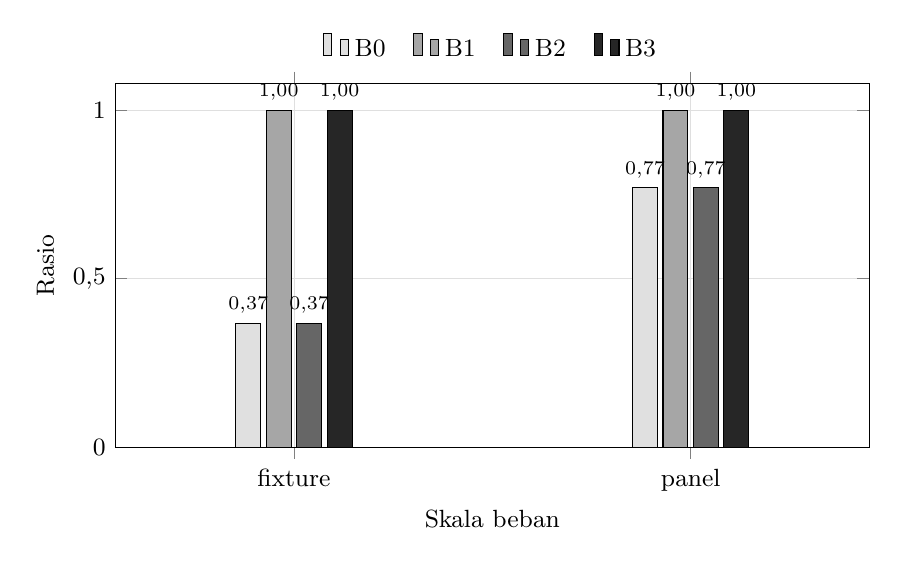
\begin{tikzpicture}
\begin{axis}[
  ybar, bar width=9pt, enlarge x limits=0.45,
  xlabel={Skala beban},
  ylabel={Rasio},
  symbolic x coords={fixture,panel},
  xtick=data, ymin=0, ymax=1.08,
  width=0.92\linewidth, height=6.2cm,
  nodes near coords={\pgfmathprintnumber[fixed, fixed zerofill, precision=2]{\pgfplotspointmeta}},
  nodes near coords style={font=\scriptsize},
  legend style={font=\small, at={(0.5,1.03)}, anchor=south, legend columns=4, draw=none, /tikz/every even column/.append style={column sep=8pt}},
  grid=major, grid style={line width=0.2pt, draw=gray!25},
  tick label style={font=\small}, label style={font=\small},
]
\addplot[draw=black, mark=none, fill=black!12] coordinates {(fixture,0.3684) (panel,0.7702)};
\addlegendentry{B0}
\addplot[draw=black, mark=none, fill=black!35] coordinates {(fixture,1.0000) (panel,1.0000)};
\addlegendentry{B1}
\addplot[draw=black, mark=none, fill=black!60] coordinates {(fixture,0.3684) (panel,0.7702)};
\addlegendentry{B2}
\addplot[draw=black, mark=none, fill=black!85] coordinates {(fixture,1.0000) (panel,1.0000)};
\addlegendentry{B3}
\end{axis}
\end{tikzpicture}
\end{document}
